\documentclass[a4paper, 12pt]{article}

\usepackage[italian]{babel}
\usepackage{verbatim}
\usepackage{graphicx}
\usepackage{float}
\usepackage[version=4]{mhchem}
\usepackage{subcaption}
\usepackage{pifont}

\linespread{1.5}



\title{Sintesi di Composti d'Interesse Medico per il Trattamento del Morbo d'Alzheimer}
\author{
	Relatrice: Annamaria DeAgostino
	\and
	Candidato: Lorenzo Castellino
}
\date{Anno Accademico 2018-2019}

\begin{document}
\pagenumbering{gobble}
\maketitle
\setcounter{page}{0}
\newpage
\tableofcontents
\newpage
\pagenumbering{arabic}

\section{Introduzione al Morbo d'Alzheimer}
La malattia di Alzheimer-Perusini, nota più comunemente come morbo d'Alzheimer (AD), è una tra le forme più diffuse al mondo di demenza senile. Dal punto di vista medico la patologia è definita come "disturbo neurocognitivo maggiore o lieve dovuto a malattia di Alzheimer".\cite{american_psychiatric_association_diagnostic_2013}
I sintomi associati sono differenti da individuo ad individuo, in generale nei pazienti riconosciuti si sono osservate:
\begin{enumerate}
	\item Perdita di memoria a breve termine.
	\item Difficoltà a concentrarsi, organizzarsi e di pianificazione.
	\item Difficoltà a seguire e/o formulare discorsi di senso compiuto.
	\item Difficoltà a giudicare distanze e spazi.
	\item Perdita di orientamento spaziale e temporale.
	\item Cambi repentini dell'umore.
	\item Allucinazioni visive.
\end{enumerate}
La demenza è una patologia di tipo progressivo, ovvero si ha un peggiormento dei sintomi col passare del tempo. La velocità di tale processo varia da persona a persona, tendenzialmente l'aspettativa media di vita successiva alla diagnosi della condizione va dai 3 ai 10 anni. \cite{todd_survival_2013}

\subsection{L'Importanza della Ricerca}
L'incidenza dell'AD è in aumento tanto da individuare la ricerca di una cura come una delle sfide per il nuovo millenio: stando al World Alzheimer Report del 2018, stilato dall'Alzheimer's Disease International ovvero l'associazione internazionale per la lotta all'Alzheimer in stretta collaborazione con la World Health Organization, si stima che nel mondo circa 50 milioni di persone siano affette da demenza. Ciò si traduce in una spesa annua per il trattamento dei malati che rasenta il miliardo di dollari.

Con l'aumento dell'aspettativa media di vita si prevede che nel 2050 il numero di casi sarà il triplo di quello odierno e si prospetta una spesa doppia rispetto a quella attuale.\cite{noauthor_world_2018}

Stando a queste previsioni 1'individuo su 85 nel 2050 sarà affetto da demenza.

L'individuazione delle cause che portano al presentarsi dell'AD è uno dei punti salienti della ricerca in campo medico e biochimico e molte sono state le ipotesi portate avanti a riguardo. Al momento una delle tesi più avvalorate e studiate è quella della formazione di aggregati proteici nel liquido cerebrospinale.

\subsection{$\beta$-Amiloidi e Placche Amiloidiche}
\label{sec:ab}
Con il termine $\beta$-amiloide (A$\beta$) si indica un frammento proteico insolubile non ramificato; tale nome è dovuto al fatto che al momento della scoperta, viste le sue proprietà si pensò in ad una similitudine con le molecole d'amido benchè dal punto di vista della composizione chimica non ci siano particolari somiglianze.\cite{lennarz_encyclopedia_2004}

L'origine di queste strutture è legata all'azione congiunta di tre enzimi ($\alpha$-secretasi,$\beta$-secretasi e $\gamma$-secretasi) su di un substrato proteico noto come APP (Amyloid Precursor Protein). L'APP è una proteina trans-membrana di modeste dimensioni (circa 700 residui), viene trasportata lungo l'assone delle cellule neuronali ed il suo accumulo è focalizzato nei siti presinaptici. Il suo rilascio è regolato dall'attività elettrica cerebrale, si suppone infatti che abbia un ruolo fondamentale nella regolazione dell'eccitabilità neuronale.\cite{mattson_cellular_1997}
La porzione che interessa la formazione di A$\beta$ è situata nel dominio extracellulare dell'APP. Come si può osservare nella Figura \ref{fig:app} i tre enzimi sopracitati agiscono in punti ben definiti e tra loro differenti della proteina; in particolare si osserva come l'azione dell'$\alpha$-secretasi non porti alla formazione del frammento $\beta$A mentre l'azione dell'enzima $\beta$ in congiunzione all'enzima $\gamma$ generi la particolare sequenza.\cite{goedert_century_2006}

\begin{figure}[H]
	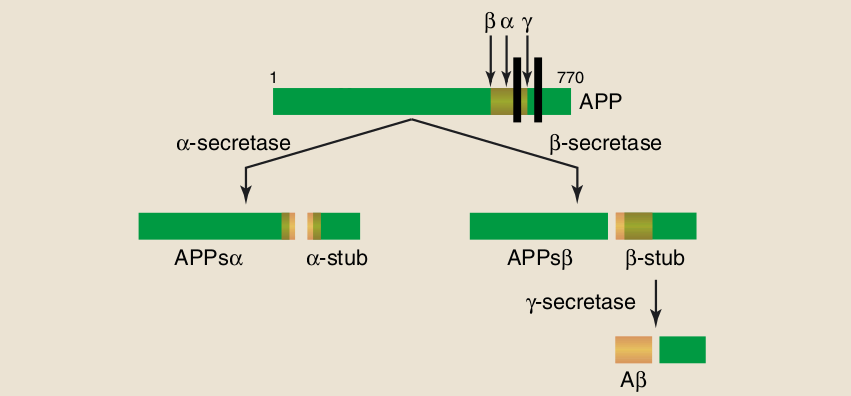
\includegraphics[width=\linewidth]{immagini/APP.png}
	\caption{Azione degli enzimi $\alpha$/$\beta$/$\gamma$-secretasi sul substrato APP.}
	\label{fig:app}
\end{figure}

I frammenti prodotti sono di due varietà che si differenziano per il numero di residui in essi contenuti, ecco quindi che possiamo distinguere i A$\beta$-40 e i A$\beta$-42 rispettivamente formati da 40 e 42 amminoacidi. Il rapporto tra le quantità prodotte delle due forme é di particolare importanza in quanto la $\beta$A-42 tende a formare oligomeri e fibrille più facilmente rispetto all’$\beta$A-40 molto probabilmente vista la minore solubilità data dai due residui idrofobici in più.\cite{kepp_bioinorganic_2012, irvine_protein_2008}

La produzione di $\beta$ in piccole quantità é un processo normale; delle funzioni osservate citiamo: \cite{brothers_physiological_2018}

\begin{enumerate}
	\item Funzione antibatterica, antifunginea e antivirale.
	\item Soppressione tumorale.
	\item Meccanismo di riparazione di falle nella barriera emato-encefalica (azione simile alle piastrine nel sangue).
	\item Regolazione dell'attività sinaptica.
\end{enumerate}

Malgrado i benefici per l'organismo una sovrapproduzione di A$\beta$ o una sproporzione verso la forma contenente 42 residui associata ad uno smaltimento non efficace sembra essere una causa sufficiente per lo sviluppo precoce del Morbo d’Alzheimer. \cite{irvine_protein_2008}
La demolizione avviene parzialmente direttamente nel cervello, come abbiamo infatti visto l'$\alpha$-secretasi effettivamente rende innocui i frammenti amiloidici scindendoli in due porzioni inerti; ma una gran parte di essa è delegata ad enzimi demolitori presenti nel fegato. La diffusione del frammento proteico insolubile è regolata dal recettore proteico LRP1 il cui processo di endocitosi è contrastato dall'azione del recettore antagonista RAGE (Figura \ref{fig:bbb}).\cite{lillis_beyond_2005, dries_extracting_2012}

\begin{figure}[H]
	\centering
	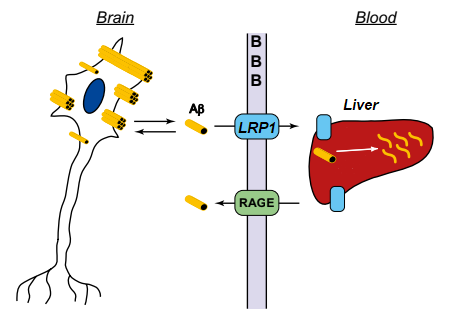
\includegraphics[width=.8\linewidth]{immagini/bbb.png}
	\caption{Fenomeno di migrazione dei A$\beta$ attraverso la barriera emato-encefalica (BBB) verso il fegato ed effetto inverso legato al recettore RAGE).}
	\label{fig:bbb}
\end{figure}

All'aumento della concentrazione di A$\beta$ nel liquido cerebrospinale è infatti associata la tendenza alla formazione di aggregati proteici più grandi ed insolubili detti comunemente "placche" o "fibrille".
L'accumulo di queste altera la chimica delle sinapsi, rallentando la trasmissione tra neuroni fino al punto di impedirla, causando così infine la morte della cellula.

Altre evidenze sperimentali mostrano come l’organismo, a causa di invecchiamento o condizioni di stress, come ad esempio la mancanza di sonno, risulta meno efficiente nella demolizione, amplificando gli effetti di accumulo nel liquido cerebrospinale.

Un'altra delle ipotesi presenta come motivo primo dell'aggregazione in placche dei frammenti A$\beta$ la presenza di concentrazioni elevate di ioni metallici nel liquido cerebrospinale. I metalli presi in esame sono Ferro, Rame e Zinco le cui concentrazioni, superato il valore di circa 10\textsuperscript{-7}  M diventano rilevanti per quanto riguarda la possibilità di essere complessati dai A$\beta$ causando una tossicità diretta o fungendo come centri iniziatori di polimerizzazione per le fibrille amiloidiche.\cite{kepp_bioinorganic_2012}

\section{Strategie d'Intervento}
Visto il complesso sistema che regola la comparsa dei A$\beta$ vien da sè che anche i metodi per cercare di limitarne la presenza o gli effetti sull'organismo saranno altrettanto variegati.

Le metodologie d'intervento studiate nel panorama della ricerca biomedica sono le più disparate. Limitandoci solo a tecniche la cui azione è incentrata direttamente sui A$\beta$ o sui loro effetti sull'organismo possiamo citare:\cite{kumar_review_2015}
\begin{enumerate}
	\item Mitigazione del trasporto dei A$\beta$ agendo sull'attività dei recettori LRP1 e RAGE.
	\item Modulazione degli enzimi responsabili della formazione di A$\beta$, in particolare modulando la demolizione tramite l'$\alpha$-secretasi o inibendo la produzione per mezzo della $\beta$-secretasi.
	\item Limitazione dell'aggregazione dei A$\beta$ in oligomeri e placche.
	\item Vaccinazione con oligomeri di A$\beta$, l'intento è quello di stimolare una risposta immunitaria all'accumularsi degli aggregati amiloidici.
	\item Modulazione della neurotrasmissione in modo da limitare l'effetto d'inibizione delle sinapsi.
	\item Mitigazione degli effetti da stress ossidativo.
\end{enumerate}

Nella seguente trattazione ci limiteremo a presentarne alcuni con esempi di composti potenzialmente interessanti dal punto di vista farmacologico soffermandoci infine in maniera più estesa su di un possibile processo di sintesi per ognuno di essi.
La discussione verterà in particolare attorno a due composti la cui azione potrebbe limitare e rallentare la neurodegenerazione nelle Sezioni \ref{sec:resv} e \ref{sec:curc}, per poi affrontare invece una possibile tecnica mirata a prevenire il presentarsi dell'AD nella Sezione \ref{sec:byp}

\section{Resveratrolo}
\label{sec:resv}
Il Resveratrolo (3,4,5'-triidrossil-trans-stilbene) è un polifenolo presente in molte piante, in particolare nella buccia e nei semi dell'uva. La sua funzione primaria nei vegetali è quella di fitoalessina, ovvero una risposta naturale nei confronti di infezioni batteriche e funginee. Alcuni studi hanno evidenziato anche diverse altre funzioni biologiche importanti come antiossidante, antinfiammatorio, fitoestrogeno e cardioprotettore.

Anche nel campo delle malattie neurodegenerative il Resveratrolo presenta alcune potenzialità; sono stati osservati effetti di riduzione dell'aggregazione dei A$\beta$ e una modulazione della neurotrasmissione mediata da Acetilcolina.

Dal punto di vista medico tale molecola è quindi un potenziale candidato per lo sviluppo di farmaci in grado di mitigare l'effetto della demenza. \cite{jabir_cholinesterase_2018}

\subsection{La Molecola}
La molecola, la cui struttura è presentata in Figura \ref{fig:resveratrolo}, è presente in natura in quantità apprezzabili in una grande varietà di piante come ad esempio le già citate bucce degli acini d'uva, ma anche in frutti con guscio, arachidi e alcune bacche. L'estrazione dai vegetali che contengono il composto, per quanto di facile realizzazione, non è sufficiente a coprire la domanda che le applicazioni in campo medico e di ricerca richiedono. Risulta quindi chiaro che lo sviluppo di un metodo di sintesi efficace e con bassi costi di realizazione sia fondamentale per rendere economicamente valida la possibilità di impiego come medicinale della molecola.
\begin{figure}[H]
	\centering
	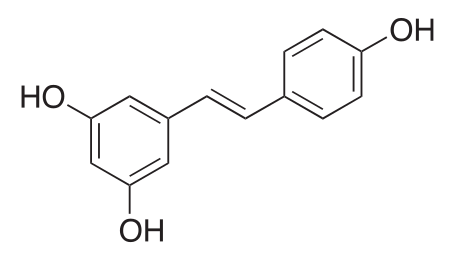
\includegraphics[width=.5\linewidth]{immagini/resveratrolo.png}
	\caption{Struttura molecolare del Resveratrolo.}
	\label{fig:resveratrolo}
\end{figure}
Oltre alla sintesi del Resveratrolo verranno presentate anche modifiche strutturali la cui presenza sembra avere un impatto positivo sull'azione del composto in casi di AD.

\subsection{Sintesi Mediante Accoppiamento Heck-Mizoroki}
Uno dei metodi più semplici ed efficaci per sintetizzare la molecola di Resveratrolo può essere realizzato mediante un accoppiamento Heck-Mizoroki. La sintesi a partire da reagenti commerciali è scomponibile in due passaggi sintetici.

\subsubsection{Reazione di Accoppiamento}
I reagenti di partenza utilizzati per l'accoppiamento sono lo 1-iodio-3,5-dimetossibenzene ed il 4-metossistirene. Il catalizzatore impiegato è un catalizzatore di palladio nanoparticellare disperso su di un supporto di argilla laponite.

La preparazione di tale dispersione viene effettuata riducendo il \ce{H2PdCl4} con etanolo in presenza di polivinilpirrolidone (PVP), il ruolo del polimero è quelo di permettere una migliore dispersione degli atomi di Palladio al fine di ottenere una migliore dispersione delle dimensioni delle nanoparticelle desiderate.

Le nanoparticelle di Palladio stabilizzate sul PVP sono quindi impregante sulla laponite lavorando in condizioni di atmosfera inerte ed utilizzando come solvente diclorometano. Il solvente viene allontanato mediante depressione; il risultato è una polvere grigia fine.\cite{martinez_extremely_2015}

Il catalizzatore così ottenuto può essere maneggiato ed utilizzato senza particolari precauzioni in reazioni atte a promuovere formazioni di legami carbonio-carbonio.

La reazione è riassunta nella Figura \ref{fig:h-m_resveratrolo}.

\begin{figure}[H]
	\centering
	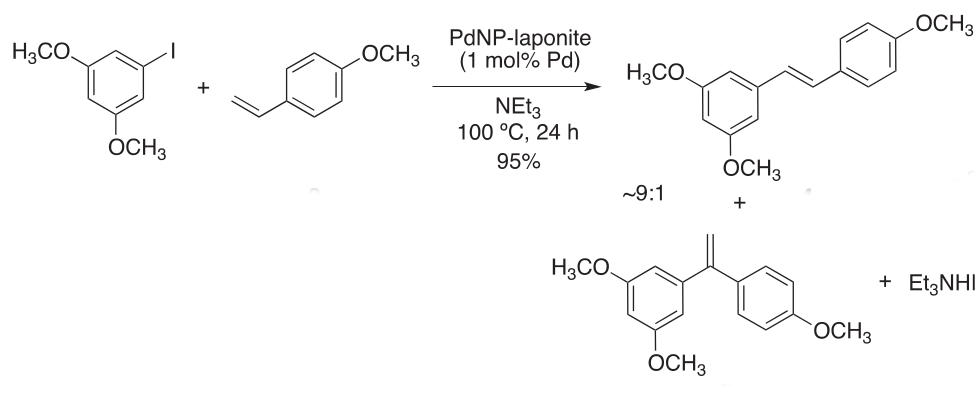
\includegraphics[width=\linewidth]{immagini/h-m_resveratrolo.png}
	\caption{Reazione di accoppiamento tra lo 1-iodio-3,5-dimetossibenzene ed il 4-metossistirene.}
	\label{fig:h-m_resveratrolo}
\end{figure}

Il ciclo catalitico è composto da quattro passaggi:
\begin{enumerate}
	\item Il catalizzatore \ce{PdL2} subisce addizione ossidativa da parte dello 1-iodio-3,5-dimetossibenzene passando da stato Pd(0) a Pd(II), ovvero da un complesso metallico a 14 elettroni ad uno a 16 elettroni.
	\item Il 4-metossistirene da carbometallazione legandosi al complesso metallico, si osserva l'inserimento del dimetossibenzene.
	\item Eliminando l'idrogeno $\beta$ i due isomeri ottenibili originati dal nuovo legame carbonio-carbonio vengono allontanati dal catalizzatore.
	\item La base forte in soluzione, in questo caso la \ce{NEt3}, ripristina il catalizzatore con Pd(0) restituendo come prodotto il composto \ce{Et3NHI}.
\end{enumerate}

La quantità di Palladio residua nei prodotti, misurata mediante analisi ad ICP-MS, risulta essere molto bassa. In una catalisi eterogenea di questo tipo è stato dimostrato che le nanoparticelle di Palladio fungono puramente da riserve di Pd(0) e che quindi la pressochè totale assenza di tracce di Palladio al termine della reazione è molto probabilmente dovuta ad un riformarsi di nanoparticelle metalliche al termine del ciclo catalitico, secondo un meccanismo di reazione catalitico "a boomerang") o ad una deposizione delle stesse sul support inorganico impiegato.

Il catalizzatore eterogeneo presenta alcuni vantaggi rispetto ad un equivalente catalizzatore omogeneo; come si può osservare in Figura \ref{fig:perc_cata_resv} il catalizzatore depositato sulla fase inorganica presenta ottime rese nei primi dieci usi. Il sottoprodotto \ce{Et3NHI} inoltre viene allontanato dal grezzo durante il decorso della reazione per deposizione dello stesso sul supporto di Laponite. D'altra parte occorre tenere conto che dopo svariati cicli di reazione la quantità di sale depositato tende ad eccedere la quantità di nanoparticelle di Palladio presenti sul supporto inficiando quindi sulla resa di reazione. Il problema è risolvibile però in maniera relativamente facile attraverso il trattamento ad alta temperatura dell'argilla di supporto. Il Trietilenammonioioduro a 550 $^\circ$C in presenza di aria subisce un processo di calcinazione; il solido restante presenta ancora una buona attività come catalizzatore nelle reazioni e può essere impiegato nuovamente per almeno tre cicli reattivi senza perdere le sue proprietà.

\begin{figure}[H]
	\centering
	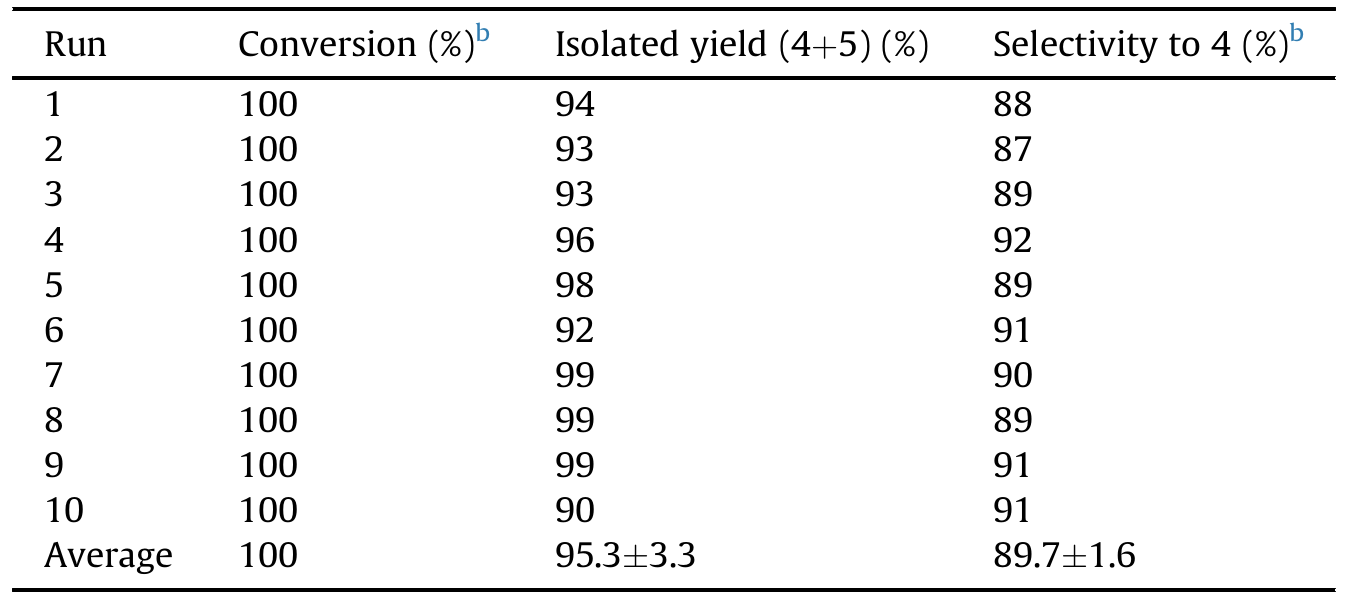
\includegraphics[width=\linewidth]{immagini/perc_cata_resv.png}
	\caption{Rese di reazione per dieci cicli catalitici successivi eseguiti utilizzando lo stesso catalizzatore. 4 = 3,4,5'-triidrossil-trans-stilbene; 5 = 3,4,5'-triidrossil-cis-stilbene}
	\label{fig:perc_cata_resv}
\end{figure}

\subsubsection{Eliminazione della Protezione Metilica}
Ai fini di ottenere la molecola di Resveratrolo è necessario rimuovere la protezione metilica presente sui gruppi metossi per ottenere sui fenoli dei gruppi idrossilici.

Tale passo sintetico è facilmente realizzabile mediante l'uso di un acido di Lewis come il Tribromuro di Bromo. Il solvente utilizzato è il Diclorometano.
La reazione è presentata in Figura \ref{fig:deprot_resveratrolo}; come si può osservare le rese per questo tipo di processo sono alte ed il processo è di facile realizzazione. \cite{alejandro_v._martinez_expedient_2017}

\begin{figure}[H]
	\centering
	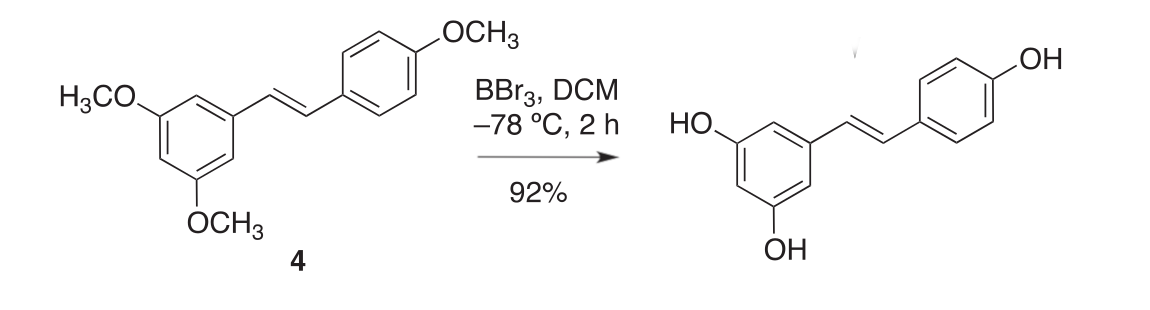
\includegraphics[width=\linewidth]{immagini/deprot_resveratrolo.png}
	\caption{Reazione di deprotezione del gruppo idrossilico sulla molecola sintetizzata.}
	\label{fig:deprot_resveratrolo}
\end{figure}

\subsection{Effetti delle Molecole Sintetizzate}
L'azione medicinale del Resveratrolo in pazienti affetti da AD è principalmente scomponibile in due componenti:

\begin{enumerate}
	\item Regolazione dell'attività neuronale.
	\item Diminuzione della citotossicità dei A$\beta$.
\end{enumerate}

La regolazione dell'attività neuronale è da ricondursi all'azione che la molecola ha nei confronti dell'enzima Acetilcolinesterasi (AChE). Tale enzima demolisce l'Acetilcolina, noto neurotrasmettitore, in Colina e Acido Acetico dopo che la molecola ha partecipato alla sinapsi tra neuroni.

\begin{figure}[H]
	\centering
	\begin{subfigure}[b]{0.4\linewidth}
		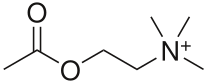
\includegraphics[width=\linewidth]{immagini/acetilcolina.png}
		\subcaption{Acetilcolina}
	\end{subfigure}
	~
	\begin{subfigure}[b]{0.4\linewidth}
		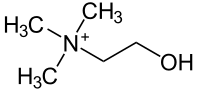
\includegraphics[width=\linewidth]{immagini/colina.png}
		\subcaption{Colina}
	\end{subfigure}
	\label{fig:coline}
\end{figure}

In casi di AD la nurotrasmissione viene ridotta in efficacia a causa dell'accumulo degli aggregati amiloidici più volte citati; ecco quindi che la normale azione dell'AChE risulta essere troppo aggressivo e la molecola di Acetilcolina rischia di essere demolita prima di aver stimolato il neurone recettore.

Il Resveratrolo funge da inibitore dell'AChE, in particolare l'inibizione è promossa da alcuni suoi oligomeri, come ad esempio la Vitisina A e lo Heyneanol A le cui strutture sono riportate in Figura \ref{fig:oly_resveratrolo}.

\begin{figure}[H]
	\centering
	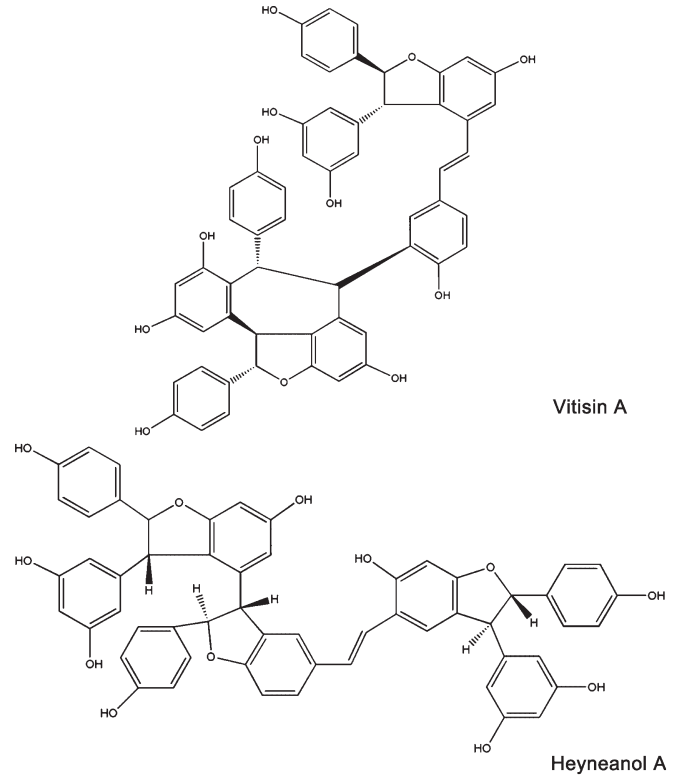
\includegraphics[width=\linewidth]{immagini/oly_resveratrolo.png}
	\caption{Struttura degli oligomeri del Resveratrolo.}
	\label{fig:oly_resveratrolo}
\end{figure}

L'azione di tali composti in presenza dell'enzima è stata osservata mediante un biotest HPLC applicato alla soluzione di enzima in presenza di diverse concentrazioni di presunto inibitore. I risultati sono riportati in Figura \ref{fig:ris_resveratrolo}. \cite{jang_inhibition_2008}

\begin{figure}[H]
	\centering
	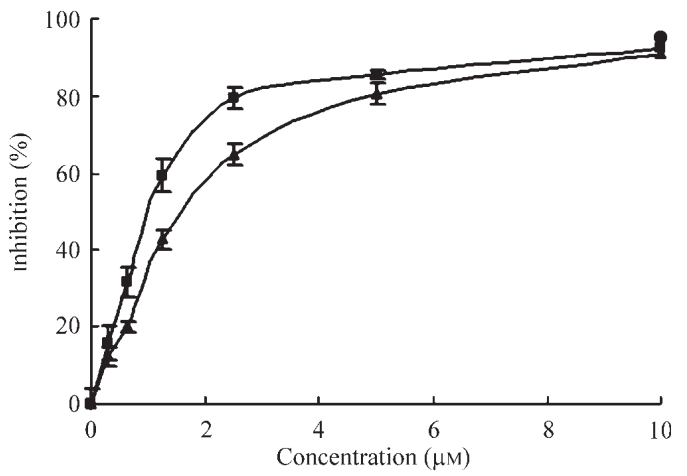
\includegraphics[width=.9\linewidth]{immagini/ris_resveratrolo.png}
	\caption{Percentuale d'inibizione dell'attività dell'enzima AChE per i composti Vitisina A (\ding{110}) e Heyneanol A (\ding{115}). }
	\label{fig:ris_resveratrolo}
\end{figure}

Il secondo metodo d'azione del Resveratrolo è legato, come anticipato sopra, ad una diminuzione della tossicità dei depositi proteici di A$\beta$. In particolare l'azione osservata è una diminuzione nel numero di fenomeni di  apoptosi nelle cellule neuronali e un ridursi in concentrazione di specie reattive ossidanti (ROI) nocive per l'organismo la cui formazione è promossa dalle fibrille stesse.

Gli esperimenti condotti ai fini di avvalorare l'importanza dal punto di vista medico del composto sono stati eseguiti utilizzando cellule della serie PC12, cellule di feocromocitoma di ratto. Gli esperimenti condotti hanno evidenziato una marcata diminuzione dei fenomeni di morte per apoptosi (Figura \ref{fig:apo_resveratrolo}) e una diminuzione in concentrazione delle specie ROI 

\section{Curcumina}
\label{sec:curc}

\section{Leganti Bipiridinici}
\label{sec:byp}
Andiamo ora a considerare una classe di composti la cui azione non è legata alla regolazione dell'attività ormonale ma ad una mitigazione del fenomeno d'aggregazione in placche dei A$\beta$. Come presentato nella Sezione \ref{sec:ab} uno dei meccanismi di aggregazione considerati alla base della formazione degli agglomerati proteici neurotossici prevede che il formarsi di un complesso tra metalli in concentrazioni sopra la norma nel liquido cerebrospinale e i A$\beta$ stessi.

L'idea alla base di un trattamento agente su questo meccanismo prevede una diminuzione dei metalli biodisponibili attraverso una chelazione degli stessi per mezzo di leganti organici.

\subsection{Le Molecole}
\label{sec:bpy_mol}
Per progettare una molecola in grado di svolgere il compito appena descritto occorrerà che questa soddisfi alcuni criteri:
\begin{enumerate}
	\item Capacità di complessare il metallo d'interesse.
	\item Costanti d'equilibrio elevate per quanto riguarda la forma complessata.
	\item Buona solubilità in ambiente acquoso, in modo da permettere la diffusione del composto all'interno del corpo.
	\item Buona permeabilità della barriera emato-encefalica; un composto che non soddisfi questo criterio avrà difficoltà ad essere trasferito nel liquido cerebrospinale.
\end{enumerate}
Una classe di composti le cui proprietà soddisfano i criteri appena presentati è quella dei derivati bipiridinici (Figura \ref{fig:bpy}).
Questi presentano una chelazione rapida, ovvero con k\textsubscript{f} nei confronti dei metalli d'interesse (Cu(II) e Zn(II)) di circa 7.0, grazie alla chelazione dell'atomo metallico da parte degli atomi d'azoto nei due eterocicli. Inoltre la solubilità in medium acquosi è relativamente buona, stiamo parlando di circa 5,9 mg/mL; infine le dimensioni ridotte permettono una buona diffusione nel sistema nervoso permeando attravero la barriera emato-encefalica con discreta facilità (i valori di permeabilità possono essere stimati attraverso le regole empiriche di Lipinski o attraverso test in vitro). \cite{di_high_2003}
\begin{figure}[H]
	\centering
	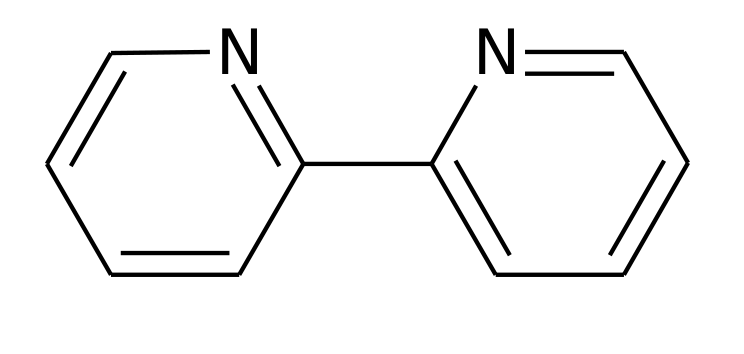
\includegraphics[width=.3\linewidth]{immagini/bpy.png}
	\caption{Un generico composto appartenente alla classe delle Bipiridine.}
	\label{fig:bpy}
\end{figure}
Lo scheletro bipiridinico ben si presta ad un approccio razionale nella sinstesi di composti interessanti dal punto di vista biomedico.
L'introduzione di gruppi dimetilamminici favorisce un'interazione con i A$\beta$ e per la sua influenza sul legame metallico come suggerito da alcune evidenze sperimentali. Similmente l'uso di un sostituente metilico permette un migliore effetto elettrodonatore da parte egli eteroatomi nei cicli e un controllo sterico sui possibili orientamenti con cui la molecola bipiridinica può interagire con il metallo. \cite{derrick_importance_2016,savelieff_ongoing_2014}

Ai fini di dimostrare l'effetto di queste modificazioni a partire dalla struttura di base sull'azione di inibizione alla formazione e disfacimento di placche amiloidiche useremo quattro prodotti di sintesi, presentati nella loro struttura in Figura \ref{fig:bpy_mod}; nella sezione successiva andremo quindi a presentare un possibile processo sintetico per essi.

\begin{figure}[H]
	\centering
	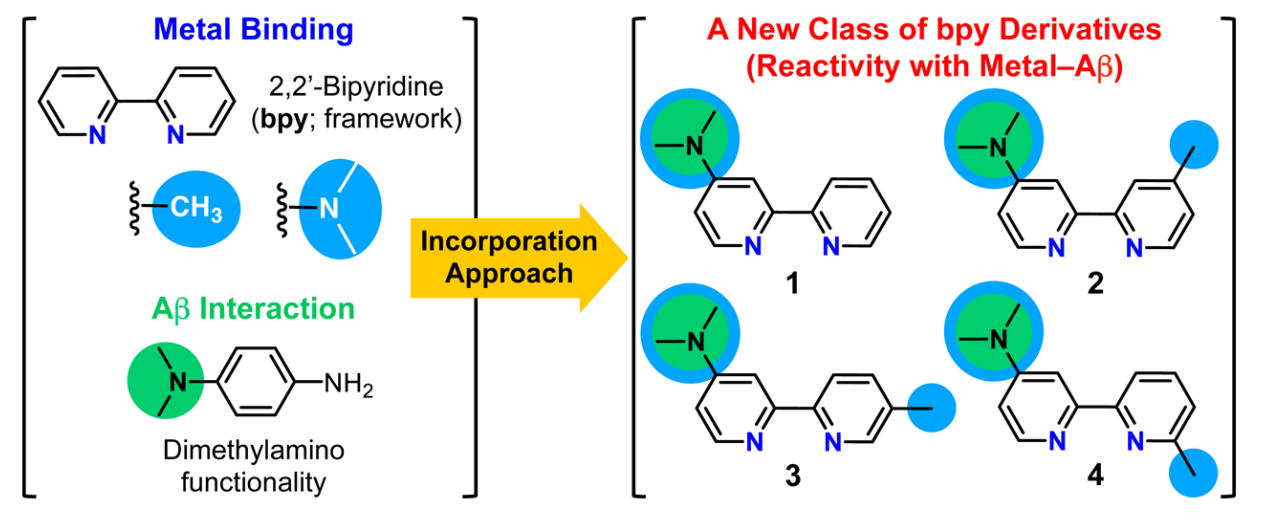
\includegraphics[width=\linewidth]{immagini/bpy_mod.png}
	\caption{Funzionalità introdotte sullo scheletro bipiridinico ai fini di ottenere i composti d'interesse 1-4}
	\label{fig:bpy_mod}
\end{figure}

\subsection{Sintesi Mediante Reazione di Stille}
\label{sec:bpy_stille}
Il processo di sintesi utilizzato è riassunto in maniera sintetica nella Figura \ref{fig:rea_g}; a partire da una 4-amminopiridina si ottiene un composto organometallico allo stagno; successivamente per mezzo di una reazione di Stille si addiziona il primo anello al secondo ottenendo il prodotto desiderato.

\begin{figure}[H]
	\centering
	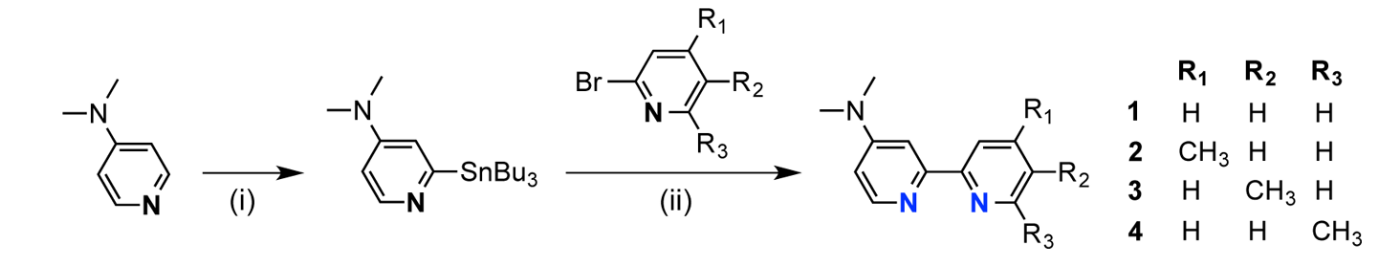
\includegraphics[width=\linewidth]{immagini/rea_g.png}
	\caption{Reazione generale per l'ottenimento dei composti d'interesse 1-4. (i) n-BuLi, 2-Dimetilaminoetanolo, Esano, 0 $^\circ$C; \ce{Bu3SnCl}, -78 $^\circ$C; (ii) \ce{PdCl2(PPh3)2}, \ce{LiCl}, \ce{PPh3}, Toluene, 110 $^\circ$C }
	\label{fig:rea_g}
\end{figure}

\subsubsection{Reazione di Formazione dello Stannano }
Il reagente di partenza, ovvero la 4-dimetilamminopiridina, viene trattata con \ce{n-BuLi} al fine di deprotonare il protone in posizione orto rispetto all'atomo di azoto presente nell'anello, il processo è noto con il nome di orto-litiazione. Lo stannano è ottenuto per transmetallazione dell'organolitiato; il \ce{Bu3SnCl} reagisce con il substrato sostituendosi all'atomo di \ce{Li} il quale si lega al \ce{Cl}.

È importante notare come la soluzione venga mantenuta a basse temperature (-78 $^\circ$C) affinchè la reazione di deprotonazione abbia luogo nel sito desiderato e che il composto organolitiato ottenuto sia sufficentemente stabile in modo tale da permettere la sostituzione con lo Stagno.
\begin{comment}
La reazione viene eseguita come segue:
\begin{enumerate}
	\item Ad una soluzione di 2-Dimetilaminoetanolo (146 mg, 1.64 mmol) in Esano (4 mL) a -5 $^\circ$C è aggiunto goccia a goccia una soluzione 2 M di \ce{n-BuLi} (1.7 mL, 3.28 mmol), si tiene in miscelazione per 30 minuti a 0 $^\circ$C sotto atmosfera d'azoto.
	\item La soluzione è trattata con 4-dimetilamminopiridina (100 mg, 0.8 mmol), miscelata per un’ora a 0 $^\circ$C e poi raffreddata a -78 $^\circ$C.
	\item Dopo l'aggiunta del \ce{Bu3SnCl} (533 mg, 1.64 mmol) la miscela di reazione è mantenuta in agitazione per 1 ora alla temperatura di 0 $^\circ$C.
	\item La reazione viene portata a termine con l'aggiunta di acqua, questa viene successivamente allontanata mediante un'estrazione in etere, il processo d'estrazione viene eseguito 3 volte. La soluzione estratta viene anidrificata con \ce{MgSO4}, filtrata e concentrata sotto vuoto.
	\item Il prodotto viene purificato in colonna cromatografica usando come eluente Acetato d'Etile (\ce{EtOAc}).
\end{enumerate}
\end{comment}


\subsubsection{Reazione di Stille per Formazione del Prodotto Finale}
Il secondo step per l'ottenimento dei composti bipiridinici d'interesse prevede una reazione di Stille, ovvero una reazione di cross-coupling palladio-catalizzata, nel caso particolare preso in esame, tra lo stannano ottenuto come prodotto dello step di reazione precedente e un alogenuro alchilico piridinico.\cite{clayden_organic_2012}

Il processo catalitico generale è riportato in maniera schematica in Figura \ref{fig:stille}.

\begin{figure}[H]
	\centering
	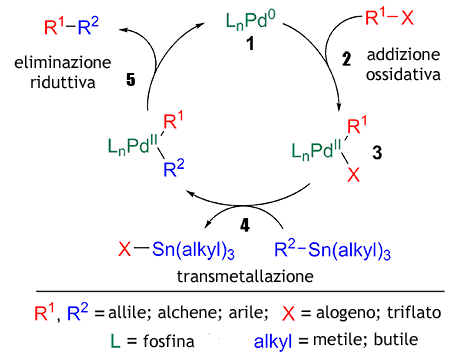
\includegraphics[width=.9\linewidth]{immagini/stille.png}
	\caption{Rappresentazione schematica del ciclo catalitico coinvolto in una reazione di Stille. Nel caso in esame R\textsuperscript{1}=2-bromopiridina, 2-bromo-4-metilpiridina, 2-bromo-5-metilpiridina, 2-bromo-6-metilpiridina R\textsuperscript{2}=N,N-dimetil-2-(tributilstannil)-piridin-4-ammina.}
	\label{fig:stille}
\end{figure}

In Toluene sono introdotti lo stannano, prodotto di reazione del passaggio sintetico precedente, il catalizzatore al palladio \ce{PdCl2(PPh3)2}, Trifenilfosfina e Cloruro di Litio. A seconda del composto bipiridinico desiderato come prodotto finale viene infine introdotta l'appropiata piridina bromurata.

Il ciclo catalitico può essere riassunto in cinque step:
\begin{enumerate}
	\item Il catalizzatore \ce{PdCl2(PPh3)2} viene ridotto a \ce{Pd(PPh3)2}, un complesso a 14 elettroni in cui il Pd ha stato d'ossidazione 0.
	\item Il complesso subisce addizione ossidativa da parte dell'alogenuro: si tratta di un processo concertato che forma un complesso a 16 elettroni con i due nuovi leganti in posizione cis.
	\item Si osserva un equilibrio d'isomerizzazione tra la forma cis e trans del complesso organometallico. La forma trans è favorita dal punto di vista termodinamico visto l'ingombro sterico originato dai leganti \ce{PPh3}.
	\item Si ha transmetallazione tra lo stannano in soluzione ed il complesso; il risultato è il trasferimento del composto arilico sul complesso con allontanamento dell'alogenuro.
	\item Un processo di eliminazione riduttiva libera il composto bipiridinico ripristinando il catalizzatore; da qui il ciclo ricomincia.
\end{enumerate}

La reazione viene condotta sotto atmosfera inerte d'Azoto per evitare che il catalizzatore possa essere alterato dalle componenti dell'aria.

\begin{comment}
Dal punto di vista operativo il processo di sintesi prosegue a partire dal prodotto isolato dalla reazione precedente:

\begin{enumerate}
	\item La N,N-dimetil-2-(tributilstannil)-piridin-4-ammina viene sciolta in Toluene (95 mg, 0.23 mmol di stannano in 2.5mL di Toluene).
	\item Sotto atmosfera inerte d'Azoto viene aggiunto il catalizzatore \ce{PdCl2(PPh3)2} (8 mg, 0.0115 mmol), il Cloruro di Litio (29 mg, 0.69 mmol), la Trifenilfosfina (6 mg, 0.023 mmol) e il bromide appropriato al prodotto desiderato (2-bromopiridina (1), 2-bromo-n-metilpiridina con n=4,5,6 (2,3,4)).
	\item La miscela è riscaldata a 110 $^\circ$C per 24 ore.
	\item I prodotti vengono purificati in colonna cromatografica.
\end{enumerate}
Nella Tabella \ref{table:stille} sono indicate le miscele usate per l'eluizione nello Step 4 e le rese ottenuta per i composti 1-4 , la numerazione segue quella espressa in Figura \ref{fig:bpy_mod}.
\begin{center}
	\begin{table}[H]
		\begin{tabular}{| c | c | c | c | }
			\hline
			Composto & \ce{EtOAc} : \ce{NEt3} & Resa \% \\	\hline
			1        & 95 : 5                 & 50 \%   \\	\hline
			2        & 99 : 1                 & 33 \%   \\	\hline
			3        & 99 : 1                 & 42 \%   \\	\hline
			4        & 99 : 1                 & 38 \%   \\	\hline
		\end{tabular}
		\centering
		\caption{Tabella contenente le rese e la composizione dell'eluente riferiti ai composti 1-4.}
		\label{table:stille}
	\end{table}
\end{center}
\end{comment}

\subsection{Sintesi Mediante Accoppiamento di Negishi}
Un metodo alternativo per la sintesi dei  bipiridinici d'interesse sfrutta la reazione di accoppiamento di Negishi. Si tratta di una reazione di accoppiamento tra un composto organozincato e un alogenuro, nel nostro caso una piridina alogenata. \cite{clayden_organic_2012}

A differenza della Reazione di Stille proposta nella Sezione \ref{sec:bpy_stille} in cui l'accoppiamento viene promosso da un composto organostannato l'uso di Zinco, la cui tossicità è nota per essere inferiore rispetto a quella dello Stagno. Il maggiore inconveniente della reazione di accoppiameno di Negishi è la sensibilità all'esposizione all'aria e all'acqua oltre ad una minore tolleranza circa il tipo di gruppi funzionali con cui è possibile lavorare.\cite{nicolaou_palladium-catalyzed_2005}

\subsubsection{Formazione del Precursore Organozincato}
Come per la formazione dello stannano il processo


\subsection{Effetti delle Molecole Sintetizzate sui A$\beta$}
L'efficacia dei composti ottenuti rispetto all'aggregazione dei A$\beta$ è stata quantificata attraverso esperimenti in vitro. I risultati sono riportati nella Figura \ref{fig:ris_bpy} per quanto riguarda l'azione in presenza di A$\beta$-40 e nella Figura \ref{fig:ris_bpy2} per il caso di A$\beta$-42.

\begin{figure}[H]
	\centering
	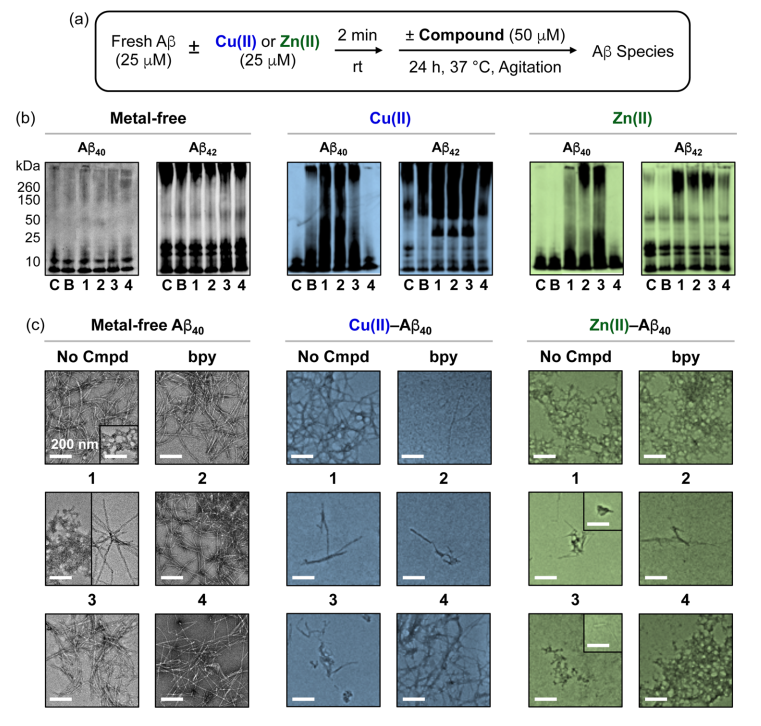
\includegraphics[width=\linewidth]{immagini/ris_bpy.png}
	\caption{(a) schematica rappresentazione della metodologia di sperimentazione; (b) corse elettroforetiche per la visualizzazione della dimensionalità delle specie A$\beta$\-40 e A$\beta$\-42 per mezzo di tecnica immunofissativa \cite{kurien_western_2006}; (c) immagini ottenute al microscopio elettronico a trasmissione (TEM) dai campioni incubati per 24 ore. C=A$\beta$+M, B=C+bpy, 1=C+1, 2=C+2, 3=C+3, 4=C+4 }
	\label{fig:ris_bpy}
\end{figure}

\begin{figure}[H]
	\centering
	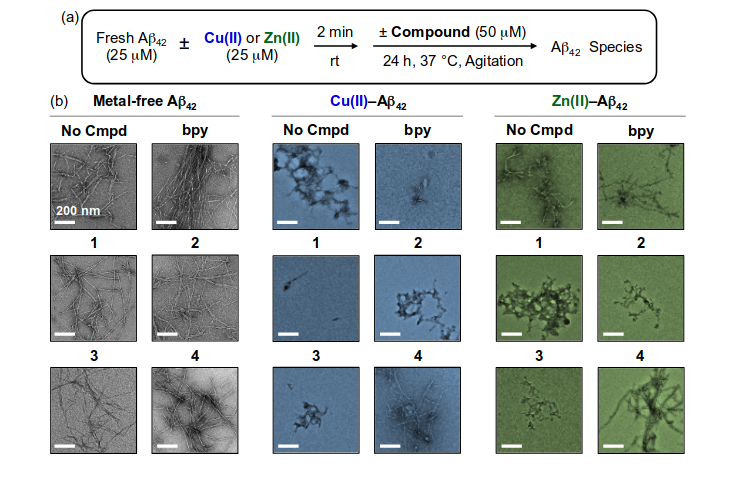
\includegraphics[width=\linewidth]{immagini/ris_bpy2.png}
	\caption{(a) schematica rappresentazione della metodologia di sperimentazione; (b) immagini ottenute al microscopio elettronico a trasmissione (TEM) dai campioni incubati per 24 ore. C=A$\beta$+M, B=C+bpy, 1=C+1, 2=C+2, 3=C+3, 4=C+4 }
	\label{fig:ris_bpy2}
\end{figure}

Nalle corse elettroforetiche mostrate in Figura \ref{fig:ris_bpy}, sezione (b), si osserva come la dimensione degli aggregati proteici tenda a diminuire in presenza dei composti sintetizzati agenti su soluzioni contenenti ioni metallici, mentre in assenza di centro di nucleazione metallico non vi siano apprezzabili effetti di mitigazione dell'accrescimento della placca. Questo è un dato atteso, i composti progettati hanno infatti lo specifico compito di chelare metalli per diminuire il fenomeno d'aggregazione, logico quindi osservare come in assenza di ioni non vi siano benefici evidenti.

Soffermandoci sulle immagine ottenute al TEM possiamo vedere come l'azione del semplice scheletro bipiridinico (bpy) modifichi l'aggregazione in presenza di Cu(II) ma non abbia evidenti effetti se confrontata con il campione C in presenza di Zn(II). I composti sintetizzati senza gruppo metilico (1) e quelli con il gruppo metilico in posizioni Meta o Para (2 e 3) hanno invece inibito la formazione di conglomerati di A$\beta$\-40 e A$\beta$\-42 sia in presenza di Cu(II) sia di Zn(II).

Il composto 4, ovvero quello con il gruppo metilico in posizione Orto non ha alterato l’aggregazione dei filamenti proteici in nessuna delle situazioni ricreate in vitro. Si tratta di un risultato atteso in quanto l’ingombro sterico del gruppo \ce{CH3} impedisce la chelazione del metallo libero che può quindi risulta disponibile come centro di nucleazione.

Benché le molecole sintetizzate risultino efficaci nella chelazione dei metalli liberi responsabili dell’accrescimento dei grumi di A$\beta$ e che la loro capacità di permeare la barriera necessaria per entrare in circolazione nel liquido cerebrospinale sia confermata da evidenze scientifiche (come già evidenziato nella Sezione \ref{sec:bpy_mol}), un test della tossicità su cellule di tipo Y5 ha evidenziato livelli notevoli di citotossicità in situazioni ci concentrazioni millimolari di Rame(II), stimolando quindi Apoptosi neuronale e vanificando quindi la possibilità di un'azione diretta come farmaco dei composti in questione.

È comunque importante considerare i risultati ottenuti, si è infatti osservato come la diminuzione degli ioni metalli biodisponibili sia un metodo efficace (almeno in vitro) per limitare l'aggregazione in fibrille dei A$\beta$ e che quindi la ricerca di composti la cui tossicità per l'organismo sia inferiore pur mantenendo simili proprietà possa essere una via promettente per il futuro. \cite{ji_strategic_2017}




\newpage




\bibliographystyle{acm}
\bibliography{biblio.bib}
\end{document}
